\documentclass[twoside]{book}

% Packages required by doxygen
\usepackage{fixltx2e}
\usepackage{calc}
\usepackage{doxygen}
\usepackage[export]{adjustbox} % also loads graphicx
\usepackage{graphicx}
\usepackage[utf8]{inputenc}
\usepackage{makeidx}
\usepackage{multicol}
\usepackage{multirow}
\PassOptionsToPackage{warn}{textcomp}
\usepackage{textcomp}
\usepackage[nointegrals]{wasysym}
\usepackage[table]{xcolor}

% Font selection
\usepackage[T1]{fontenc}
\usepackage[scaled=.90]{helvet}
\usepackage{courier}
\usepackage{amssymb}
\usepackage{sectsty}
\renewcommand{\familydefault}{\sfdefault}
\allsectionsfont{%
  \fontseries{bc}\selectfont%
  \color{darkgray}%
}
\renewcommand{\DoxyLabelFont}{%
  \fontseries{bc}\selectfont%
  \color{darkgray}%
}
\newcommand{\+}{\discretionary{\mbox{\scriptsize$\hookleftarrow$}}{}{}}

% Page & text layout
\usepackage{geometry}
\geometry{%
  a4paper,%
  top=2.5cm,%
  bottom=2.5cm,%
  left=2.5cm,%
  right=2.5cm%
}
\tolerance=750
\hfuzz=15pt
\hbadness=750
\setlength{\emergencystretch}{15pt}
\setlength{\parindent}{0cm}
\setlength{\parskip}{3ex plus 2ex minus 2ex}
\makeatletter
\renewcommand{\paragraph}{%
  \@startsection{paragraph}{4}{0ex}{-1.0ex}{1.0ex}{%
    \normalfont\normalsize\bfseries\SS@parafont%
  }%
}
\renewcommand{\subparagraph}{%
  \@startsection{subparagraph}{5}{0ex}{-1.0ex}{1.0ex}{%
    \normalfont\normalsize\bfseries\SS@subparafont%
  }%
}
\makeatother

% Headers & footers
\usepackage{fancyhdr}
\pagestyle{fancyplain}
\fancyhead[LE]{\fancyplain{}{\bfseries\thepage}}
\fancyhead[CE]{\fancyplain{}{}}
\fancyhead[RE]{\fancyplain{}{\bfseries\leftmark}}
\fancyhead[LO]{\fancyplain{}{\bfseries\rightmark}}
\fancyhead[CO]{\fancyplain{}{}}
\fancyhead[RO]{\fancyplain{}{\bfseries\thepage}}
\fancyfoot[LE]{\fancyplain{}{}}
\fancyfoot[CE]{\fancyplain{}{}}
\fancyfoot[RE]{\fancyplain{}{\bfseries\scriptsize Generated by Doxygen }}
\fancyfoot[LO]{\fancyplain{}{\bfseries\scriptsize Generated by Doxygen }}
\fancyfoot[CO]{\fancyplain{}{}}
\fancyfoot[RO]{\fancyplain{}{}}
\renewcommand{\footrulewidth}{0.4pt}
\renewcommand{\chaptermark}[1]{%
  \markboth{#1}{}%
}
\renewcommand{\sectionmark}[1]{%
  \markright{\thesection\ #1}%
}

% Indices & bibliography
\usepackage{natbib}
\usepackage[titles]{tocloft}
\setcounter{tocdepth}{3}
\setcounter{secnumdepth}{5}
\makeindex

% Hyperlinks (required, but should be loaded last)
\usepackage{ifpdf}
\ifpdf
  \usepackage[pdftex,pagebackref=true]{hyperref}
\else
  \usepackage[ps2pdf,pagebackref=true]{hyperref}
\fi
\hypersetup{%
  colorlinks=true,%
  linkcolor=blue,%
  citecolor=blue,%
  unicode%
}

% Custom commands
\newcommand{\clearemptydoublepage}{%
  \newpage{\pagestyle{empty}\cleardoublepage}%
}

\usepackage{caption}
\captionsetup{labelsep=space,justification=centering,font={bf},singlelinecheck=off,skip=4pt,position=top}

%===== C O N T E N T S =====

\begin{document}

% Titlepage & ToC
\hypersetup{pageanchor=false,
             bookmarksnumbered=true,
             pdfencoding=unicode
            }
\pagenumbering{roman}
\begin{titlepage}
\vspace*{7cm}
\begin{center}%
{\Large Thimblerigger -\/ Perception Challenge \\[1ex]\large 1.\+0.\+0 }\\
\vspace*{1cm}
{\large Generated by Doxygen 1.8.11}\\
\end{center}
\end{titlepage}
\clearemptydoublepage
\tableofcontents
\clearemptydoublepage
\pagenumbering{arabic}
\hypersetup{pageanchor=true}

%--- Begin generated contents ---
\chapter{Thimblerigger Challenge of the N\+RP}
\label{md_README}
\hypertarget{md_README}{}
This repository defines the challenge perception \char`\"{}\+Thimblerigger\char`\"{}. It is part of the K\+IT course \char`\"{}\+Virtual Neurorobotics\char`\"{}.

This repo is for the {\bfseries challenge definition} only, to create a solution please fork this repository and implement your solution there.

\subsection*{Installing}

Assuming that you have a local install of the \href{https://bitbucket.org/hbpneurorobotics/neurorobotics-platform}{\tt N\+RP}, no special setup is needed. Simply fork this repo into the {\bfseries Experiments} folder. When starting the N\+RP frontend, you should now see an experiment called {\bfseries Perception\+Challenge\+K\+IT}.

\subsection*{Running the experiment}

Start the experiment. You will be in a paused state with nothing in the world but an i\+Cub Robot. Once you hit the play button, three red cylinders will spawn in front of the robot. These cylinders represent 3 mugs. One of the mugs contains a green ball. The goal of the challenge is to\+:


\begin{DoxyItemize}
\item Check which mug contains the ball
\item Track that mug during shuffling. Shuffling computes {\itshape n} random permutations of the mug order and moves the mugs into the corresponding positions. At most 2 mugs are displaced at one time, one to either side of the original lane.
\item Tell which mug contains the ball in any way, e.\+g.\+: Publish an index, point the robot to the correct mug, ...
\end{DoxyItemize}

\subsection*{Interacting with the experiment}

The user can manually navigate through the challenge by sending the following R\+OS service requests. You can do this via command line, or {\ttfamily rospy.\+Service\+Proxy} objects. (The challenge does nothing if you do not send these requests, it is an \char`\"{}interactive\char`\"{} challenge)\+:

\tabulinesep=1mm
\begin{longtabu} spread 0pt [c]{*3{|X[-1]}|}
\hline
\rowcolor{\tableheadbgcolor}{\bf Service name }&{\bf Service Type }&{\bf Description  }\\\cline{1-3}
\endfirsthead
\hline
\endfoot
\hline
\rowcolor{\tableheadbgcolor}{\bf Service name }&{\bf Service Type }&{\bf Description  }\\\cline{1-3}
\endhead
/thimblerigger/reset&std\+\_\+srvs/\+Trigger&Despawns the mugs, respawns them in the starting sorted order and chooses a new mug under which the ball is contained \\\cline{1-3}
/thimblerigger/show\+\_\+correct\+\_\+mug&std\+\_\+srvs/\+Trigger&Lifts up the mug under which the ball is contained and shows the ball \\\cline{1-3}
/thimblerigger/hide\+\_\+correct\+\_\+mug&std\+\_\+srvs/\+Trigger&Hides the ball again under the mug if it was lifted up \\\cline{1-3}
/thimblerigger/shuffle&std\+\_\+srvs/\+Trigger&Randomly permutes the mugs n times. n is a parameter of the thimblerigger challenge. \\\cline{1-3}
\end{longtabu}
You can also use a stepping mechanism (implemented in the state machine)\+:

\tabulinesep=1mm
\begin{longtabu} spread 0pt [c]{*3{|X[-1]}|}
\hline
\rowcolor{\tableheadbgcolor}{\bf Service name }&{\bf Service Type }&{\bf Description  }\\\cline{1-3}
\endfirsthead
\hline
\endfoot
\hline
\rowcolor{\tableheadbgcolor}{\bf Service name }&{\bf Service Type }&{\bf Description  }\\\cline{1-3}
\endhead
/thimblerigger/start\+\_\+challenge&std\+\_\+srvs/\+Trigger&Once the simulation is running, starts the thimblerigger state machine \\\cline{1-3}
/thimblerigger/step\+\_\+challenge&std\+\_\+srvs/\+Trigger&Steps through the challenge in this order (one step per service call)\+: {\ttfamily Show correct mug -\/ Hide correct mug -\/ Shuffle -\/ Show correct mug -\/ (Then the state machine exits, feel free to implement a loop/reset mechanism)} \\\cline{1-3}
/thimblerigger/stop\+\_\+challenge&std\+\_\+srvs/\+Trigger&Currently not used \\\cline{1-3}
\end{longtabu}
\subsubsection*{Training signal}

There is a training signal for supervised training being published under the topic {\ttfamily /thimblerigger/training\+\_\+signal}. It publishes the index of the correct mug, as soon as it is known (meaning before the {\ttfamily /thimblerigger/show\+\_\+correct\+\_\+mug} service is called, a $\ast$-\/1$\ast$ is published).

The 3 indices {\ttfamily \mbox{[}0, 1, 2\mbox{]}} are arranged as follows\+: {\ttfamily 0} is closest to the default robot starting position, {\ttfamily 2} the furthest away. If you reset the challenge with the service call, the training signal will be reset, too. The index switches every time the mug has reached its goal position during shuffling, but not in between.

\subsubsection*{Auto-\/stepper}

If you don\textquotesingle{}t want/need to manually trigger the different stages of the challenge via the R\+OS service calls, there is an auto-\/stepper which can automatically trigger the stages of the challenge for you. It is implemented in stepper.\+py. To use it, simply uncomment the last two lines in the state machine.

\subsection*{What am I allowed to modify?}

\subsubsection*{What you shouldn\textquotesingle{}t modify}

There is a configuration file {\ttfamily thimblerigger\+\_\+config.\+py}, that allows to configure things like topic names. The paragraph above assumes that you have not changed those.

You should not fiddle with the following files (and any references to one of these files in any configuration file)\+:


\begin{DoxyItemize}
\item {\ttfamily state\+\_\+machine.\+exd}
\item {\ttfamily stepper.\+py}
\item {\ttfamily thimblerigger\+\_\+server.\+py}
\item {\ttfamily thimblerigger.\+py} (this is where most interesting stuff happens)
\end{DoxyItemize}

Feel free to read through them for further information how the challenge works internally, the {\ttfamily thimblerigger$\ast$.py} files are well documented. You can find doxygen pages in the {\ttfamily docs} folder.

\subsubsection*{Things that you should definitely change}

In {\ttfamily bibi\+\_\+configuration.\+bibi}\+:


\begin{DoxyItemize}
\item There is a {\ttfamily file}-\/tag within {\ttfamily brain\+Model} that points to a file that load the brain of the robot. This is relative to the {\itshape Models} folder in the N\+RP. On a local install, it is best to create a new file within the experiment repo, and put a path relative to the {\itshape Models} directory in this tag. (This is to avoid splitting the solution into multiple repos). For example\+: 
\begin{DoxyCode}
1 <\textcolor{keywordtype}{brainModel}>
2     <\textcolor{keywordtype}{file}>../\textcolor{keyword}{Experiments}/\textcolor{keyword}{hbpprak\_perception}/\textcolor{keyword}{my\_custom\_brain.py}</\textcolor{keywordtype}{file}>
3 </\textcolor{keywordtype}{brainModel}>
\end{DoxyCode}
 will allow you to have the brain file within your solution fork of the challenge repo.
\item Add transfer functions, spike recorders, etc. in the bibi file, see \href{https://developer.humanbrainproject.eu/docs/projects/HBP%20Neurorobotics%20Platform/1.2/nrp/tutorials/transfer_function/bibi_config.html}{\tt the documentation}.
\end{DoxyItemize}

\subsubsection*{Things that you might want to change}

In {\ttfamily thimblerigger\+\_\+config.\+py}\+:
\begin{DoxyItemize}
\item {\itshape num\+\_\+mugs}, {\itshape num\+\_\+shuffles} and {\itshape seed}. The final challenge uses 3 cups, 1 shuffle, and the seed for shuffling and choice of which mug contains the ball should be random (i.\+e. {\ttfamily seed = None}).
\end{DoxyItemize}

Additionally, you might want to modify\+:

In {\ttfamily Ex\+D\+Perception\+Challenge\+K\+I\+T.\+exc}\+:


\begin{DoxyItemize}
\item The timeout in seconds (for debugging). Default is 10 minutes.
\item The robot starting position ({\ttfamily robot\+Pose}-\/tag)
\end{DoxyItemize}

\subsection*{Additional Information}


\begin{DoxyItemize}
\item \href{https://youtu.be/aice0elP7eI}{\tt Demo video}
\item \href{https://bitbucket.org/hbpneurorobotics/neurorobotics-platform}{\tt N\+RP}
\item \href{https://forum.humanbrainproject.eu/}{\tt N\+RP Forum}
\item \href{http://wiki.ros.org/ROS/Tutorials/WritingServiceClient%28python%29#rospy_tutorials.2BAC8-Tutorials.2BAC8-WritingServiceClient.Writing_the_Client_Node}{\tt Rospy service clients} 
\end{DoxyItemize}
\chapter{Hierarchical Index}
\section{Class Hierarchy}
This inheritance list is sorted roughly, but not completely, alphabetically\+:\begin{DoxyCompactList}
\item object\begin{DoxyCompactList}
\item \contentsline{section}{stepper.\+Stepper}{\pageref{classstepper_1_1Stepper}}{}
\item \contentsline{section}{thimblerigger.\+Thimblerigger}{\pageref{classthimblerigger_1_1Thimblerigger}}{}
\item \contentsline{section}{thimblerigger\+\_\+server.\+Thimblerigger\+Challenge\+Server}{\pageref{classthimblerigger__server_1_1ThimbleriggerChallengeServer}}{}
\end{DoxyCompactList}
\end{DoxyCompactList}

\chapter{Class Index}
\section{Class List}
Here are the classes, structs, unions and interfaces with brief descriptions\+:\begin{DoxyCompactList}
\item\contentsline{section}{\hyperlink{classstepper_1_1Stepper}{stepper.\+Stepper} }{\pageref{classstepper_1_1Stepper}}{}
\item\contentsline{section}{\hyperlink{classthimblerigger_1_1Thimblerigger}{thimblerigger.\+Thimblerigger} }{\pageref{classthimblerigger_1_1Thimblerigger}}{}
\item\contentsline{section}{\hyperlink{classthimblerigger__server_1_1ThimbleriggerChallengeServer}{thimblerigger\+\_\+server.\+Thimblerigger\+Challenge\+Server} }{\pageref{classthimblerigger__server_1_1ThimbleriggerChallengeServer}}{}
\end{DoxyCompactList}

\chapter{Class Documentation}
\hypertarget{classstepper_1_1Stepper}{}\section{stepper.\+Stepper Class Reference}
\label{classstepper_1_1Stepper}\index{stepper.\+Stepper@{stepper.\+Stepper}}


Inheritance diagram for stepper.\+Stepper\+:\nopagebreak
\begin{figure}[H]
\begin{center}
\leavevmode
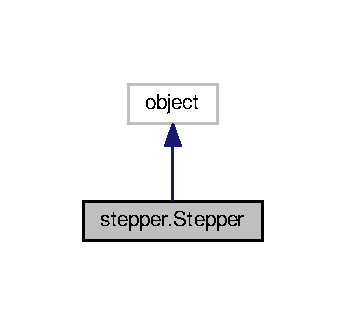
\includegraphics[width=166pt]{classstepper_1_1Stepper__inherit__graph}
\end{center}
\end{figure}


Collaboration diagram for stepper.\+Stepper\+:\nopagebreak
\begin{figure}[H]
\begin{center}
\leavevmode
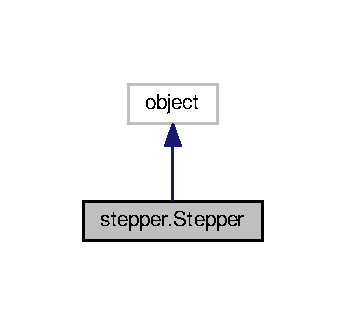
\includegraphics[width=166pt]{classstepper_1_1Stepper__coll__graph}
\end{center}
\end{figure}
\subsection*{Public Member Functions}
\begin{DoxyCompactItemize}
\item 
def {\bfseries \+\_\+\+\_\+init\+\_\+\+\_\+} (self)\hypertarget{classstepper_1_1Stepper_aaad0869347ab473e035679f01f296790}{}\label{classstepper_1_1Stepper_aaad0869347ab473e035679f01f296790}

\item 
def {\bfseries run\+\_\+async} (self)\hypertarget{classstepper_1_1Stepper_aa5a2d8c11f92fdf6a81182cbed4a758c}{}\label{classstepper_1_1Stepper_aa5a2d8c11f92fdf6a81182cbed4a758c}

\end{DoxyCompactItemize}
\subsection*{Public Attributes}
\begin{DoxyCompactItemize}
\item 
{\bfseries process}\hypertarget{classstepper_1_1Stepper_a66d8fe911e06db3ea2e2b0ff7d423291}{}\label{classstepper_1_1Stepper_a66d8fe911e06db3ea2e2b0ff7d423291}

\end{DoxyCompactItemize}


\subsection{Detailed Description}
\begin{DoxyVerb}Dummy object for spawning a separate process for stepping through the challenge.
This is only useful for debugging the step mode. Later, calling the step
service will be done by the team solving the challenge.
\end{DoxyVerb}
 

The documentation for this class was generated from the following file\+:\begin{DoxyCompactItemize}
\item 
stepper.\+py\end{DoxyCompactItemize}

\hypertarget{classthimblerigger_1_1Thimblerigger}{}\section{thimblerigger.\+Thimblerigger Class Reference}
\label{classthimblerigger_1_1Thimblerigger}\index{thimblerigger.\+Thimblerigger@{thimblerigger.\+Thimblerigger}}


Inheritance diagram for thimblerigger.\+Thimblerigger\+:\nopagebreak
\begin{figure}[H]
\begin{center}
\leavevmode
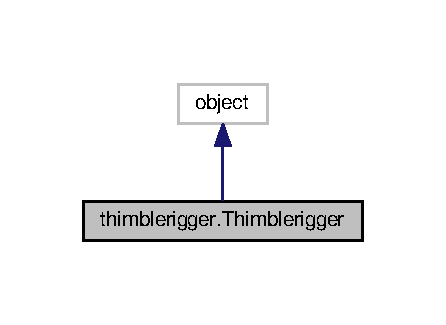
\includegraphics[width=214pt]{classthimblerigger_1_1Thimblerigger__inherit__graph}
\end{center}
\end{figure}


Collaboration diagram for thimblerigger.\+Thimblerigger\+:\nopagebreak
\begin{figure}[H]
\begin{center}
\leavevmode
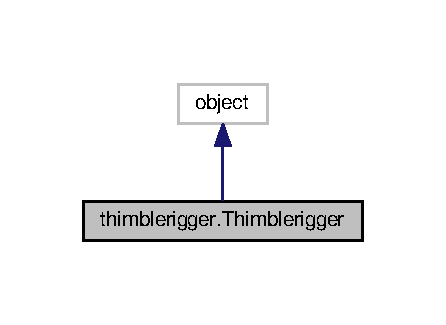
\includegraphics[width=214pt]{classthimblerigger_1_1Thimblerigger__coll__graph}
\end{center}
\end{figure}
\subsection*{Public Member Functions}
\begin{DoxyCompactItemize}
\item 
def \hyperlink{classthimblerigger_1_1Thimblerigger_a34788bd8195b1ebd76e76a0eb665ee18}{\+\_\+\+\_\+init\+\_\+\+\_\+} (self, num\+\_\+mugs=3, num\+\_\+shuffles=1, mug\+\_\+radius=0.\+1, mug\+\_\+height=0.\+15, seed=None, movement\+\_\+rate=None)
\item 
def \hyperlink{classthimblerigger_1_1Thimblerigger_a7198939b327adbba670b58b310556d05}{reset} (self)
\item 
def \hyperlink{classthimblerigger_1_1Thimblerigger_aece869c0bf0650d676c9d171224a929e}{choose\+\_\+mug\+\_\+for\+\_\+ball} (self)
\item 
def \hyperlink{classthimblerigger_1_1Thimblerigger_acc7947cf77d97be49bb797783a21c671}{show\+\_\+mug\+\_\+with\+\_\+ball} (self)
\item 
def \hyperlink{classthimblerigger_1_1Thimblerigger_a508a70bc68cb5f8fa4b01ddecf584de5}{hide\+\_\+ball\+\_\+under\+\_\+mug} (self)
\item 
def {\bfseries shuffle} (self)\hypertarget{classthimblerigger_1_1Thimblerigger_aebfd2a3be6761c6ce4e3c9c12111ee85}{}\label{classthimblerigger_1_1Thimblerigger_aebfd2a3be6761c6ce4e3c9c12111ee85}

\end{DoxyCompactItemize}
\subsection*{Public Attributes}
\begin{DoxyCompactItemize}
\item 
{\bfseries mug\+\_\+sdf}\hypertarget{classthimblerigger_1_1Thimblerigger_ad7bde60a4a4100106b35aeea7a8bdc4d}{}\label{classthimblerigger_1_1Thimblerigger_ad7bde60a4a4100106b35aeea7a8bdc4d}

\item 
{\bfseries ball\+\_\+sdf}\hypertarget{classthimblerigger_1_1Thimblerigger_a554e7cc6a5ba0c4e015b57e5547dc77e}{}\label{classthimblerigger_1_1Thimblerigger_a554e7cc6a5ba0c4e015b57e5547dc77e}

\item 
{\bfseries rnd}\hypertarget{classthimblerigger_1_1Thimblerigger_ac03059436234f63e9a7363812d931ffe}{}\label{classthimblerigger_1_1Thimblerigger_ac03059436234f63e9a7363812d931ffe}

\item 
{\bfseries start\+\_\+position}\hypertarget{classthimblerigger_1_1Thimblerigger_a5ddc1158ae68104b270d9cc5329b00f5}{}\label{classthimblerigger_1_1Thimblerigger_a5ddc1158ae68104b270d9cc5329b00f5}

\item 
{\bfseries mug\+\_\+order}\hypertarget{classthimblerigger_1_1Thimblerigger_a22086a4a32882f909b1058b3c6470416}{}\label{classthimblerigger_1_1Thimblerigger_a22086a4a32882f909b1058b3c6470416}

\item 
{\bfseries num\+\_\+shuffles}\hypertarget{classthimblerigger_1_1Thimblerigger_a421e6c23e3be10b762c1cdf40a07237c}{}\label{classthimblerigger_1_1Thimblerigger_a421e6c23e3be10b762c1cdf40a07237c}

\item 
{\bfseries mug\+\_\+height}\hypertarget{classthimblerigger_1_1Thimblerigger_a0a98ffc00195a655191250aea282684b}{}\label{classthimblerigger_1_1Thimblerigger_a0a98ffc00195a655191250aea282684b}

\item 
{\bfseries mug\+\_\+radius}\hypertarget{classthimblerigger_1_1Thimblerigger_a61c50d73706348c76493ad9698074267}{}\label{classthimblerigger_1_1Thimblerigger_a61c50d73706348c76493ad9698074267}

\item 
{\bfseries lift\+\_\+height}\hypertarget{classthimblerigger_1_1Thimblerigger_a0025d86bbbe9654c6d4178ae537671f6}{}\label{classthimblerigger_1_1Thimblerigger_a0025d86bbbe9654c6d4178ae537671f6}

\item 
{\bfseries shuffle\+\_\+displacement}\hypertarget{classthimblerigger_1_1Thimblerigger_a82156fb2f87051aa557e849009fa3726}{}\label{classthimblerigger_1_1Thimblerigger_a82156fb2f87051aa557e849009fa3726}

\item 
{\bfseries ball\+\_\+radius}\hypertarget{classthimblerigger_1_1Thimblerigger_a78d0df2afc03a5b6286715d9e386f1f8}{}\label{classthimblerigger_1_1Thimblerigger_a78d0df2afc03a5b6286715d9e386f1f8}

\item 
{\bfseries movement\+\_\+rate}\hypertarget{classthimblerigger_1_1Thimblerigger_a3b7c954f3f4ad08807d5b72f021af561}{}\label{classthimblerigger_1_1Thimblerigger_a3b7c954f3f4ad08807d5b72f021af561}

\item 
{\bfseries mug\+\_\+with\+\_\+ball\+\_\+intermediate\+\_\+index}\hypertarget{classthimblerigger_1_1Thimblerigger_ab7b7fe3d00cc03647329282ed765456c}{}\label{classthimblerigger_1_1Thimblerigger_ab7b7fe3d00cc03647329282ed765456c}

\item 
{\bfseries mug\+\_\+with\+\_\+ball}\hypertarget{classthimblerigger_1_1Thimblerigger_a9fec172e829583bfe6c1f31c719b933d}{}\label{classthimblerigger_1_1Thimblerigger_a9fec172e829583bfe6c1f31c719b933d}

\item 
{\bfseries send\+\_\+training\+\_\+signal}\hypertarget{classthimblerigger_1_1Thimblerigger_ac83105705969ba7f738050440c3777fc}{}\label{classthimblerigger_1_1Thimblerigger_ac83105705969ba7f738050440c3777fc}

\end{DoxyCompactItemize}


\subsection{Constructor \& Destructor Documentation}
\index{thimblerigger\+::\+Thimblerigger@{thimblerigger\+::\+Thimblerigger}!\+\_\+\+\_\+init\+\_\+\+\_\+@{\+\_\+\+\_\+init\+\_\+\+\_\+}}
\index{\+\_\+\+\_\+init\+\_\+\+\_\+@{\+\_\+\+\_\+init\+\_\+\+\_\+}!thimblerigger\+::\+Thimblerigger@{thimblerigger\+::\+Thimblerigger}}
\subsubsection[{\texorpdfstring{\+\_\+\+\_\+init\+\_\+\+\_\+(self, num\+\_\+mugs=3, num\+\_\+shuffles=1, mug\+\_\+radius=0.\+1, mug\+\_\+height=0.\+15, seed=\+None, movement\+\_\+rate=\+None)}{__init__(self, num_mugs=3, num_shuffles=1, mug_radius=0.1, mug_height=0.15, seed=None, movement_rate=None)}}]{\setlength{\rightskip}{0pt plus 5cm}def thimblerigger.\+Thimblerigger.\+\_\+\+\_\+init\+\_\+\+\_\+ (
\begin{DoxyParamCaption}
\item[{}]{self, }
\item[{}]{num\+\_\+mugs = {\ttfamily 3}, }
\item[{}]{num\+\_\+shuffles = {\ttfamily 1}, }
\item[{}]{mug\+\_\+radius = {\ttfamily 0.1}, }
\item[{}]{mug\+\_\+height = {\ttfamily 0.15}, }
\item[{}]{seed = {\ttfamily None}, }
\item[{}]{movement\+\_\+rate = {\ttfamily None}}
\end{DoxyParamCaption}
)}\hypertarget{classthimblerigger_1_1Thimblerigger_a34788bd8195b1ebd76e76a0eb665ee18}{}\label{classthimblerigger_1_1Thimblerigger_a34788bd8195b1ebd76e76a0eb665ee18}
\begin{DoxyVerb}Thimblerigger is a game challenge for the NRP simulator.
There are some mugs on the ground.
The robot is shown a ball under one of the mugs.
Then, the mugs are shuffled.
In the end, the robot has to identify which mug the ball is under.

:param num_mugs: Number of mugs to spawn.
:param num_shuffles: Number of permutations to go through when shuffling once.
:param mug_radius: Radius for one mug.
:param mug_height: Height of one mug.
All movements will scale to fit the radius and height parameters.
:param seed: Seed for the random number generator controlling which mug the ball is under
     and what shuffling permutations are generated.
:param movement_rate: Rate in Hz which is used to publish to movement topics, e.g. shuffling the mugs.
              A lower rate will wait longer between intermediate steps.
              Use this to control the time if you brain simulation is slow.
\end{DoxyVerb}
 

\subsection{Member Function Documentation}
\index{thimblerigger\+::\+Thimblerigger@{thimblerigger\+::\+Thimblerigger}!choose\+\_\+mug\+\_\+for\+\_\+ball@{choose\+\_\+mug\+\_\+for\+\_\+ball}}
\index{choose\+\_\+mug\+\_\+for\+\_\+ball@{choose\+\_\+mug\+\_\+for\+\_\+ball}!thimblerigger\+::\+Thimblerigger@{thimblerigger\+::\+Thimblerigger}}
\subsubsection[{\texorpdfstring{choose\+\_\+mug\+\_\+for\+\_\+ball(self)}{choose_mug_for_ball(self)}}]{\setlength{\rightskip}{0pt plus 5cm}def thimblerigger.\+Thimblerigger.\+choose\+\_\+mug\+\_\+for\+\_\+ball (
\begin{DoxyParamCaption}
\item[{}]{self}
\end{DoxyParamCaption}
)}\hypertarget{classthimblerigger_1_1Thimblerigger_aece869c0bf0650d676c9d171224a929e}{}\label{classthimblerigger_1_1Thimblerigger_aece869c0bf0650d676c9d171224a929e}
\begin{DoxyVerb}Chooses a new mug for the ball to be under.

:returns None.
\end{DoxyVerb}
 \index{thimblerigger\+::\+Thimblerigger@{thimblerigger\+::\+Thimblerigger}!hide\+\_\+ball\+\_\+under\+\_\+mug@{hide\+\_\+ball\+\_\+under\+\_\+mug}}
\index{hide\+\_\+ball\+\_\+under\+\_\+mug@{hide\+\_\+ball\+\_\+under\+\_\+mug}!thimblerigger\+::\+Thimblerigger@{thimblerigger\+::\+Thimblerigger}}
\subsubsection[{\texorpdfstring{hide\+\_\+ball\+\_\+under\+\_\+mug(self)}{hide_ball_under_mug(self)}}]{\setlength{\rightskip}{0pt plus 5cm}def thimblerigger.\+Thimblerigger.\+hide\+\_\+ball\+\_\+under\+\_\+mug (
\begin{DoxyParamCaption}
\item[{}]{self}
\end{DoxyParamCaption}
)}\hypertarget{classthimblerigger_1_1Thimblerigger_a508a70bc68cb5f8fa4b01ddecf584de5}{}\label{classthimblerigger_1_1Thimblerigger_a508a70bc68cb5f8fa4b01ddecf584de5}
\begin{DoxyVerb}Lowers the mug under which the ball is located so the ball is invisible.

:return True, if the mug was lowered and the ball is invisible.
\end{DoxyVerb}
 \index{thimblerigger\+::\+Thimblerigger@{thimblerigger\+::\+Thimblerigger}!reset@{reset}}
\index{reset@{reset}!thimblerigger\+::\+Thimblerigger@{thimblerigger\+::\+Thimblerigger}}
\subsubsection[{\texorpdfstring{reset(self)}{reset(self)}}]{\setlength{\rightskip}{0pt plus 5cm}def thimblerigger.\+Thimblerigger.\+reset (
\begin{DoxyParamCaption}
\item[{}]{self}
\end{DoxyParamCaption}
)}\hypertarget{classthimblerigger_1_1Thimblerigger_a7198939b327adbba670b58b310556d05}{}\label{classthimblerigger_1_1Thimblerigger_a7198939b327adbba670b58b310556d05}
\begin{DoxyVerb}Resets the state of the thimblerigger.
Specifically, it:
- Hides the ball
- Chooses a new mug for the ball to be under

:returns True.
\end{DoxyVerb}
 \index{thimblerigger\+::\+Thimblerigger@{thimblerigger\+::\+Thimblerigger}!show\+\_\+mug\+\_\+with\+\_\+ball@{show\+\_\+mug\+\_\+with\+\_\+ball}}
\index{show\+\_\+mug\+\_\+with\+\_\+ball@{show\+\_\+mug\+\_\+with\+\_\+ball}!thimblerigger\+::\+Thimblerigger@{thimblerigger\+::\+Thimblerigger}}
\subsubsection[{\texorpdfstring{show\+\_\+mug\+\_\+with\+\_\+ball(self)}{show_mug_with_ball(self)}}]{\setlength{\rightskip}{0pt plus 5cm}def thimblerigger.\+Thimblerigger.\+show\+\_\+mug\+\_\+with\+\_\+ball (
\begin{DoxyParamCaption}
\item[{}]{self}
\end{DoxyParamCaption}
)}\hypertarget{classthimblerigger_1_1Thimblerigger_acc7947cf77d97be49bb797783a21c671}{}\label{classthimblerigger_1_1Thimblerigger_acc7947cf77d97be49bb797783a21c671}
\begin{DoxyVerb}Lifts the mug under which the ball is located up and shows the ball.

:returns True, if the mug was lifted and the ball is visible.
\end{DoxyVerb}
 

The documentation for this class was generated from the following file\+:\begin{DoxyCompactItemize}
\item 
thimblerigger.\+py\end{DoxyCompactItemize}

\hypertarget{classthimblerigger__server_1_1ThimbleriggerChallengeServer}{}\section{thimblerigger\+\_\+server.\+Thimblerigger\+Challenge\+Server Class Reference}
\label{classthimblerigger__server_1_1ThimbleriggerChallengeServer}\index{thimblerigger\+\_\+server.\+Thimblerigger\+Challenge\+Server@{thimblerigger\+\_\+server.\+Thimblerigger\+Challenge\+Server}}


Inheritance diagram for thimblerigger\+\_\+server.\+Thimblerigger\+Challenge\+Server\+:\nopagebreak
\begin{figure}[H]
\begin{center}
\leavevmode
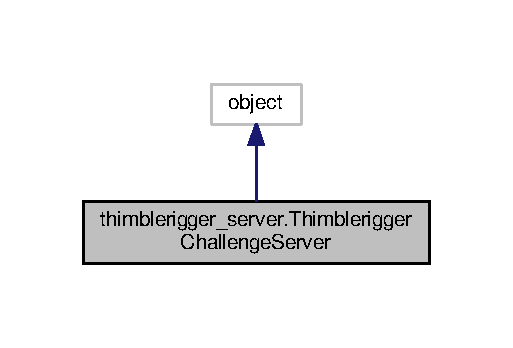
\includegraphics[width=246pt]{classthimblerigger__server_1_1ThimbleriggerChallengeServer__inherit__graph}
\end{center}
\end{figure}


Collaboration diagram for thimblerigger\+\_\+server.\+Thimblerigger\+Challenge\+Server\+:\nopagebreak
\begin{figure}[H]
\begin{center}
\leavevmode
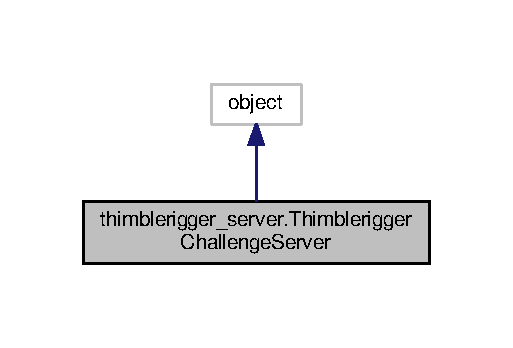
\includegraphics[width=246pt]{classthimblerigger__server_1_1ThimbleriggerChallengeServer__coll__graph}
\end{center}
\end{figure}
\subsection*{Public Member Functions}
\begin{DoxyCompactItemize}
\item 
def {\bfseries \+\_\+\+\_\+init\+\_\+\+\_\+} (self)\hypertarget{classthimblerigger__server_1_1ThimbleriggerChallengeServer_a53c52a84120d95ba74380ddb92c94c87}{}\label{classthimblerigger__server_1_1ThimbleriggerChallengeServer_a53c52a84120d95ba74380ddb92c94c87}

\item 
def \hyperlink{classthimblerigger__server_1_1ThimbleriggerChallengeServer_a949229494a1ac9dbff020430e28ab6be}{handle\+\_\+start} (self, req)
\item 
def \hyperlink{classthimblerigger__server_1_1ThimbleriggerChallengeServer_ad69a9dd2ec8e81a3482e553b809c4db8}{handle\+\_\+stop} (self, req)
\item 
def \hyperlink{classthimblerigger__server_1_1ThimbleriggerChallengeServer_a0a96eddd98d2f362bea78861e846b283}{handle\+\_\+step} (self, req)
\item 
def {\bfseries serve} (self)\hypertarget{classthimblerigger__server_1_1ThimbleriggerChallengeServer_af3c6b32e27acaa7252cd5b272e209a9e}{}\label{classthimblerigger__server_1_1ThimbleriggerChallengeServer_af3c6b32e27acaa7252cd5b272e209a9e}

\end{DoxyCompactItemize}
\subsection*{Public Attributes}
\begin{DoxyCompactItemize}
\item 
{\bfseries running}\hypertarget{classthimblerigger__server_1_1ThimbleriggerChallengeServer_a23d3ea1848ec23cd59dacf12e14f14de}{}\label{classthimblerigger__server_1_1ThimbleriggerChallengeServer_a23d3ea1848ec23cd59dacf12e14f14de}

\item 
{\bfseries challenge\+\_\+started\+\_\+pub}\hypertarget{classthimblerigger__server_1_1ThimbleriggerChallengeServer_a3c075847a889773ecc747c1890d9e303}{}\label{classthimblerigger__server_1_1ThimbleriggerChallengeServer_a3c075847a889773ecc747c1890d9e303}

\item 
{\bfseries step\+\_\+pub}\hypertarget{classthimblerigger__server_1_1ThimbleriggerChallengeServer_af86d6f03cb152026d62c8f35914795d3}{}\label{classthimblerigger__server_1_1ThimbleriggerChallengeServer_af86d6f03cb152026d62c8f35914795d3}

\end{DoxyCompactItemize}


\subsection{Member Function Documentation}
\index{thimblerigger\+\_\+server\+::\+Thimblerigger\+Challenge\+Server@{thimblerigger\+\_\+server\+::\+Thimblerigger\+Challenge\+Server}!handle\+\_\+start@{handle\+\_\+start}}
\index{handle\+\_\+start@{handle\+\_\+start}!thimblerigger\+\_\+server\+::\+Thimblerigger\+Challenge\+Server@{thimblerigger\+\_\+server\+::\+Thimblerigger\+Challenge\+Server}}
\subsubsection[{\texorpdfstring{handle\+\_\+start(self, req)}{handle_start(self, req)}}]{\setlength{\rightskip}{0pt plus 5cm}def thimblerigger\+\_\+server.\+Thimblerigger\+Challenge\+Server.\+handle\+\_\+start (
\begin{DoxyParamCaption}
\item[{}]{self, }
\item[{}]{req}
\end{DoxyParamCaption}
)}\hypertarget{classthimblerigger__server_1_1ThimbleriggerChallengeServer_a949229494a1ac9dbff020430e28ab6be}{}\label{classthimblerigger__server_1_1ThimbleriggerChallengeServer_a949229494a1ac9dbff020430e28ab6be}
\begin{DoxyVerb}Currently not used, but could be used for timing etc.
\end{DoxyVerb}
 \index{thimblerigger\+\_\+server\+::\+Thimblerigger\+Challenge\+Server@{thimblerigger\+\_\+server\+::\+Thimblerigger\+Challenge\+Server}!handle\+\_\+step@{handle\+\_\+step}}
\index{handle\+\_\+step@{handle\+\_\+step}!thimblerigger\+\_\+server\+::\+Thimblerigger\+Challenge\+Server@{thimblerigger\+\_\+server\+::\+Thimblerigger\+Challenge\+Server}}
\subsubsection[{\texorpdfstring{handle\+\_\+step(self, req)}{handle_step(self, req)}}]{\setlength{\rightskip}{0pt plus 5cm}def thimblerigger\+\_\+server.\+Thimblerigger\+Challenge\+Server.\+handle\+\_\+step (
\begin{DoxyParamCaption}
\item[{}]{self, }
\item[{}]{req}
\end{DoxyParamCaption}
)}\hypertarget{classthimblerigger__server_1_1ThimbleriggerChallengeServer_a0a96eddd98d2f362bea78861e846b283}{}\label{classthimblerigger__server_1_1ThimbleriggerChallengeServer_a0a96eddd98d2f362bea78861e846b283}
\begin{DoxyVerb}Callback for stepping through the state machine.
\end{DoxyVerb}
 \index{thimblerigger\+\_\+server\+::\+Thimblerigger\+Challenge\+Server@{thimblerigger\+\_\+server\+::\+Thimblerigger\+Challenge\+Server}!handle\+\_\+stop@{handle\+\_\+stop}}
\index{handle\+\_\+stop@{handle\+\_\+stop}!thimblerigger\+\_\+server\+::\+Thimblerigger\+Challenge\+Server@{thimblerigger\+\_\+server\+::\+Thimblerigger\+Challenge\+Server}}
\subsubsection[{\texorpdfstring{handle\+\_\+stop(self, req)}{handle_stop(self, req)}}]{\setlength{\rightskip}{0pt plus 5cm}def thimblerigger\+\_\+server.\+Thimblerigger\+Challenge\+Server.\+handle\+\_\+stop (
\begin{DoxyParamCaption}
\item[{}]{self, }
\item[{}]{req}
\end{DoxyParamCaption}
)}\hypertarget{classthimblerigger__server_1_1ThimbleriggerChallengeServer_ad69a9dd2ec8e81a3482e553b809c4db8}{}\label{classthimblerigger__server_1_1ThimbleriggerChallengeServer_ad69a9dd2ec8e81a3482e553b809c4db8}
\begin{DoxyVerb}Currently not used, but could be used for timing etc.
\end{DoxyVerb}
 

The documentation for this class was generated from the following file\+:\begin{DoxyCompactItemize}
\item 
thimblerigger\+\_\+server.\+py\end{DoxyCompactItemize}

%--- End generated contents ---

% Index
\backmatter
\newpage
\phantomsection
\clearemptydoublepage
\addcontentsline{toc}{chapter}{Index}
\printindex

\end{document}
